\sect{Matrizen}

\ssect{Definition}

Unter einer $m \times n$ \textbf{Matrix} versteht man ein rechteckiges Zahlenschema von doppelt indizierten Grössen $a_{ij}$ mit $m$ waagerecht angeordneten Zeilen und $n$ senkrecht angeordneten Spalten.

\ssect{Rechnen mit Matrizen}

\sssect{Skalare Multiplikation}

Die \textbf{skalare Multiplikation} der $m \times n$ Matrix $A$ mit dem reellen Skalar $\lambda$ ist definiert durch die elementweise Multiplikation mit der Zahl $\lambda$:
\[\lambda A = \lambda \left(
\begin{array}{ccc}
    a_{11} & \ldots & a_{1n} \\
    \vdots & \ddots & \vdots \\
    a_{m1} & \ldots & a_{mn}
\end{array}
\right) = \left(
\begin{array}{ccc}
    \lambda a_{11} & \ldots & \lambda a_{1n} \\
    \vdots         & \ddots & \vdots         \\
    \lambda a_{m1} & \ldots & \lambda a_{mn}
\end{array}
\right)\]

\textbf{Rechenregeln:}

$\lambda$ und $\mu$ sind reelle Skalare, $A$ und $B$ sind $m \times n$ Matrizen.
Dann gilt:
\begin{itemize}
    \item Assoziativgesetz: $\lambda (\mu A) = \mu (\lambda A) = (\lambda \mu) A$
    \item Distributivgesetz 1: $(\lambda + \mu) A = \lambda A + \mu A$
    \item Distributivgesetz 2: $\lambda (A + B) = \lambda A + \lambda B$
\end{itemize}

Für Matrizen $A_1, \dots, A_p$ derselben Grösse und Skalare $\lambda_1, \dots, \lambda_p$ heisst $\lambda_1 A_1 + \dots + \lambda_p A_p$ die \textbf{Linearkombination} von $A_1, \dots, A_p$ mit Koeffizienten $\lambda_1, \dots, \lambda_p$.

\sssect{Multiplikation von Matrizen}

Gegeben seien die Matrizen $A \in \R^{m \times n}$ und $B \in \R^{n \times p}$.
Die \textbf{Produktmatrix} $C = AB$ ist eine $m \times p$ Matrix:
\[c_{ij} = a_{i1} b_{1j} + \dots + a_{in} b_{nj} = \sum_{k=1}^{n} a_{ik} b_{kj}\]
Mit anderen Worten: $c_{ij}$ ergibt sich aus der $i$-te Zeile der Matrix $A$ mal die $j$-te Spalte der Matrix $B$.

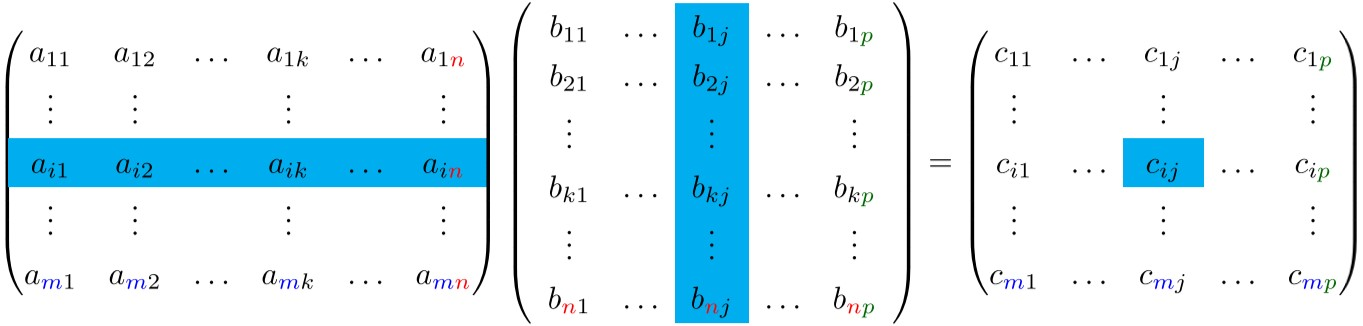
\includegraphics[scale=0.255]{dot-product}

Die Anzahl von Spalten in $A$ muss gleich der Anzahl von Zeilen in $B$ sein!

Das Matrizenprodukt ist generell \textbf{nicht kommutativ}: $AB \neq BA$!

\ssect{Inverse Matrix}

Gibt es zu einer $n \times n$ Matrix $A$ eine Matrix $X$ mit $AX = XA = I_n$, so heisst $X$ die zu $A$ inverse Matrix.
Sie wird durch das Symbol $A^{-1} gekennzeichnet.$

\textbf{Anmerkung:}
\begin{itemize}
    \item Falls eine quadratische Matrix $A$ eine Inverse $A^{-1}$ besitzt, so ist $A^{-1}$ eindeutig bestimmt.
    Die Matrix $A$ heisst in diesem Fall \textbf{invertierbar} (oder \textbf{umkehrbar}).
    Andernfalls heisst sie \textbf{singulär}.
    \item Es gilt: $AA^{-1} = A^{-1}A = I_n$.
    Das heisst, dass $A$ und $A^{-1}$ kommutativ sind.
\end{itemize}

\textbf{Satz:} Das Produkt $AB$ zweier invertierbarer Matrizen ist invertierbar.
Die Inverse zu $AB$ lautet: $(AB)^{-1} = B^{-1} A^{-1}$

\sssect{Berechnung}

Die Matrix $A = \left(
\begin{array}{cc}
    a & b \\ c & d
\end{array} \right) \in \R^{n \times n}$ ist für $\det(A) = ad - bc \neq 0$ invertierbar.
In diesem Fall gilt:
\[A^{-1} = \frac{1}{\det(A)} \left(
\begin{array}{cc}
    d & -b \\ -c & a
\end{array}
\right)\]
Für eine $n \times n$ Matrix $A$ berechnet man $A^{-1}$ wie folgt:
\begin{itemize}
    \item Wir betrachten die erweiterte Koeffizientenmatrix:
    \[(A | I_n) = \left(
    \begin{array}{cccc|cccc}
        a_{11} & a_{12} & \ldots & a_{1n} & 1      & 0      & \ldots & 0      \\
        a_{21} & a_{22} & \ldots & a_{2n} & 0      & 1      & \ldots & 0      \\
        \vdots & \vdots & \ddots & \vdots & \vdots & \vdots & \ddots & \vdots \\
        a_{n1} & a_{n2} & \ldots & a_{nm} & 0      & 0      & \ldots & 1
    \end{array}
    \right)\]
    \item Mit Gauss-Jordan-Verfahren auf reduzierte ZSF bringen.
    \item Ist der \textbf{Rang der Matrix $A$ gleich $n$}, dann lässt sich $A^{-1}$ direkt an der reduzierten ZSF ablesen.

    \[\left(
    \begin{array}{cccc|cccc}
        1      & 0      & \ldots & 0      & x_{11} & x_{12} & \ldots & x_{1n} \\
        0      & 1      & \ldots & 0      & x_{21} & x_{22} & \ldots & x_{2n} \\
        \vdots & \vdots & \ddots & \vdots & \vdots & \vdots & \ddots & \vdots \\
        0      & 0      & \ldots & 1      & x_{n1} & x_{n2} & \ldots & x_{nm}
    \end{array}
    \right) = (I_n | A^{-1})\]
    Ist der \textbf{Rang der Matrix $A$ kleiner als $n$}, dann gibt es keine Inverse.
\end{itemize}

\ssect{Transponierte Matrix}

Sei $A$ eine $m \times n$ Matrix.
Die \textbf{transponierte Matrix} $A^T$ erhält man aus $A$, indem man die $i$-te Spalte von $A$ zur $i$-ten Zeile von $A^T$ macht.
Kurz: $\left[ A^T \right]_{ij} = a_{ij}$

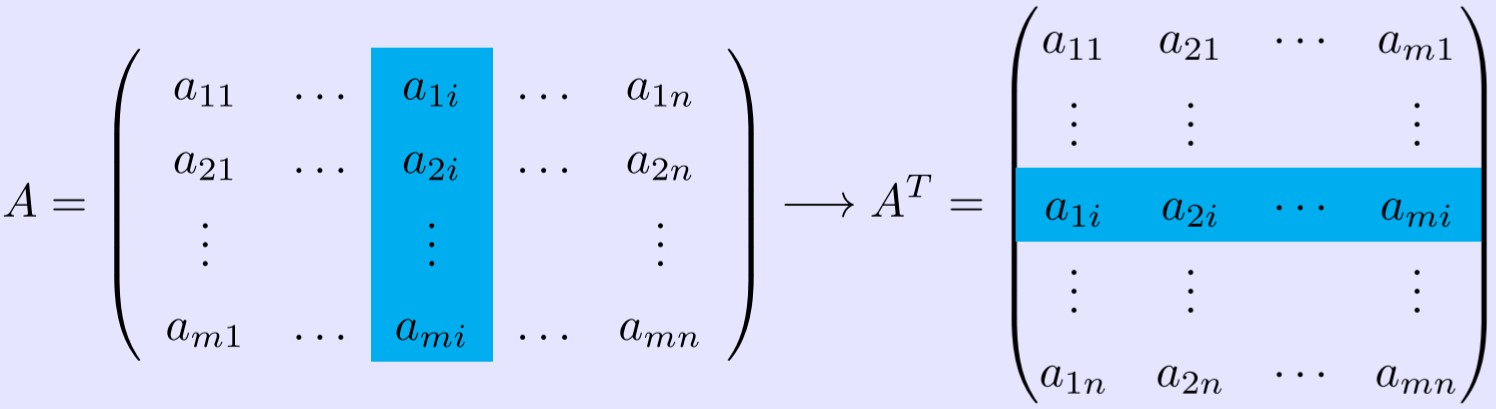
\includegraphics[scale=0.23]{transponierte}

\textbf{Anmerkung:}
\begin{itemize}
    \item Ist $A$ eine $m \times n$ Matrix, so ist ihre Transponierte $A^T$ eine $n \times m$ Matrix.
    \item $(A^T)^T = A$
    \item Durch Transponieren geht ein Zeilenvektor in einen Spaltenvektor über und umgekehrt.
    \item Es gilt für eine symmetrische Matrix $A$ stets: $A^T = A$
\end{itemize}

\textbf{Rechenregeln:}
\begin{enumerate}
    \item $(A + B)^T = A^T + B^T$ für alle $m \times n$ Matrizen $A$ und $B$.
    \item $(\lambda A)^T = \lambda A^T$ $\forall A \in \R^{m \times n}$ und $\forall \lambda \in \R$
    \item $(AB)^T = B^T A^T$ für $A \in \R^{m \times n}$ und $B \in \R^{n \times p}$
    \item $(A^T)^{-1} = (A^{-1})^T$ für eine invertierbare $n \times n$ Matrix $A$
\end{enumerate}